\section{創業進度規劃與團隊能力}

\subsection{經營團隊與組織架構}

普羅程式於2021年成立,由三位海大資工系學生組成,成員中簡蔚驊具備全端工程師專業背景,林一與王裕傑曾一同發表AI相關論文於IEEE研討會,並由海大資工的馬尚彬教授、魚樂天地鄉鎮應援團的何立德執行長分別擔任技術顧問和商業顧問。

團隊成員皆有豐富的程式設計、軟體開發、計畫執行、數位行銷等經驗,
包括參與112年學年度大專校院創業實戰模擬學習平臺之第二梯次\footnote{大專校院創業實戰模擬學習平臺(普羅程式):https://ssp.moe.gov.tw/cases/854}(圖\ref{fig:experience-1})
、提案於flyingV群眾募資平台\footnote{flyingV群眾募資平台(普羅Python入門課程):https://www.flyingv.cc/projects/29572}(圖\ref{fig:experience-2}、附件\ref{fig:Appendix-fundraising})以及經營團隊社群與網站(附件\ref{fig:Appendix-Marketing}),並於海大教學中心參與多次創業研習(附件\ref{fig:Appendix-Training})。

\begin{figure}[H]
  \centering
  \begin{subfigure}{0.45\linewidth}
    \centering
    %   \href{https://raw.githubusercontent.com/programingtw/proglearn-plan/main/img/interactiveMeterial.png}{ 
    
\includegraphics[width=0.8\textwidth]{images/maker.png}
    %   }
    \caption{大專校院創業實戰模擬學習平臺 - 提案封面}
    \label{fig:experience-1}
  \end{subfigure}
    \begin{subfigure}{0.45\linewidth}
    \centering
    %   \href{https://raw.githubusercontent.com/programingtw/proglearn-plan/main/img/interactiveMeterial2.png}{ 
    
\includegraphics[width=0.8\textwidth]{images/flyingv.jpg}
    %   }
    \caption{flyingV群眾募資 - 提案封面}
    \label{fig:experience-2}
  \end{subfigure}
  \caption{創業經歷}
  \label{fig:Experience}
\end{figure}

此外,我們曾在全國性比賽中獲得多項獎項,包括2023資訊智慧創新跨域專題競賽特優獎(圖\ref{fig:Awards-1})並登上年代新聞(圖\ref{fig:News})、2021年潮創客大賽優選獎(圖\ref{fig:Awards-2})、2021武漢金銀湖盃第七屆海峽兩岸青年創新創業大賽入選台灣賽區菁英賽決賽、2021師大Startup競技場決賽(附件\ref{fig:Appendix-Competition})。

\begin{figure}[H]
  \centering
  \begin{subfigure}{0.32\linewidth}
    \centering
    %   \href{https://raw.githubusercontent.com/programingtw/proglearn-plan/main/img/interactiveMeterial.png}{ 
    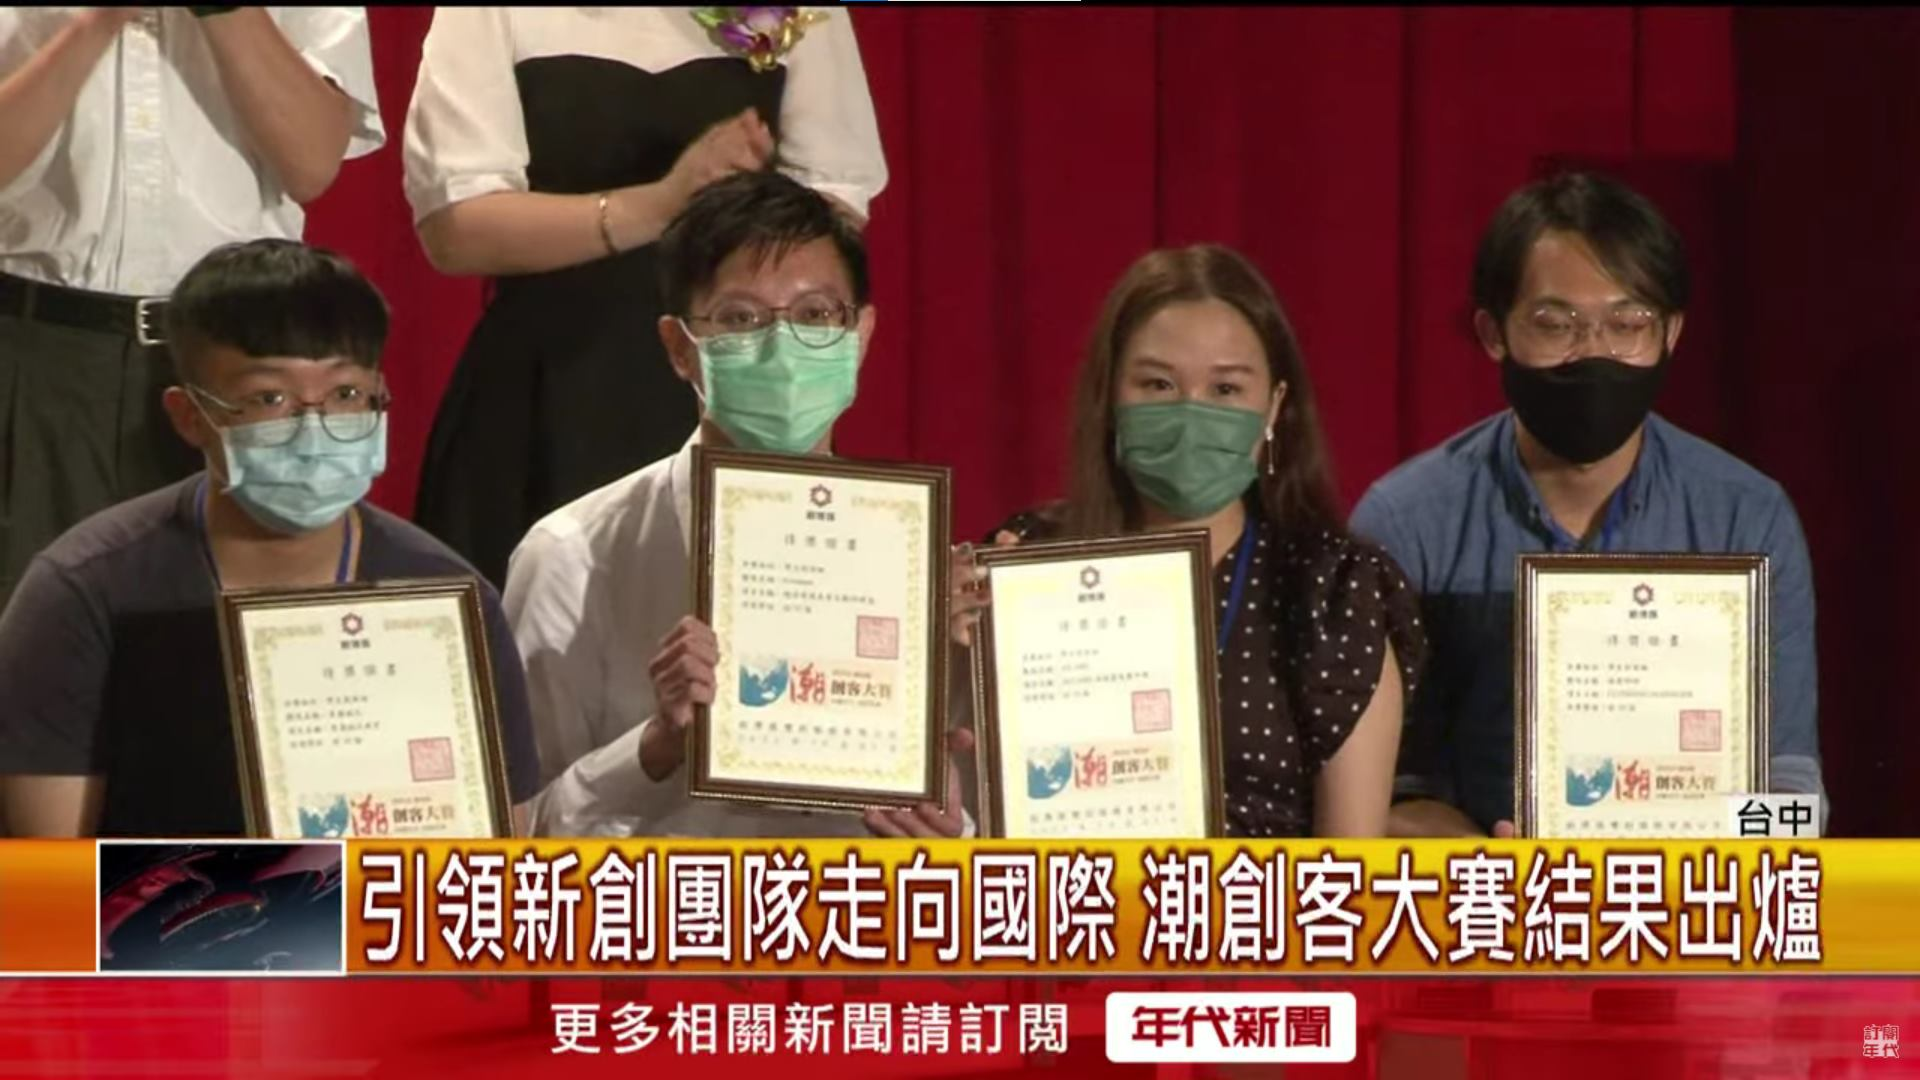
\includegraphics[width=0.8\textwidth]{images/年代新聞.jpg}
    %   }
    \caption{年代新聞}
    \label{fig:News}
  \end{subfigure}
    \begin{subfigure}{0.31\linewidth}
    \centering
    %   \href{https://raw.githubusercontent.com/programingtw/proglearn-plan/main/img/interactiveMeterial2.png}{ 
    
\includegraphics[width=0.45\textwidth]{images/ProgLearn.jpg}
    %   }
    \caption{資訊智慧創新跨域專題競賽}
    \label{fig:Awards-1}
  \end{subfigure}
  \begin{subfigure}{0.31\linewidth}
    \centering
      %   \href{https://raw.githubusercontent.com/programingtw/proglearn-plan/main/img/interactiveMeterial2.png}{ 
    
\includegraphics[width=0.45\textwidth]{images/創博匯.jpg}
      %   }
    \caption{潮創客大賽}
    \label{fig:Awards-2}
  \end{subfigure}
  \caption{團隊榮譽}
\end{figure}